\documentclass[UTF8]{ctexart}
\usepackage{subfigure}
\usepackage{caption}
\usepackage{amsmath}
\usepackage{amssymb}
\usepackage{pifont}
\usepackage{geometry}
\usepackage{graphicx}
\usepackage{gensymb}
\usepackage{wrapfig}
\usepackage{titlesec}
\usepackage{float}
\usepackage{diagbox}
\usepackage{fancyhdr}
\usepackage{color}
\pagestyle{plain}
\geometry{a4paper,scale=0.8}
\CTEXsetup[format+={\raggedright}]{section} 
\title{通网2016-2017期末}
\author{Deschain}
\titlespacing*{\section}
{0pt}{0pt}{0pt}
\titlespacing*{\subsection}
{0pt}{0pt}{0pt}
\titlespacing*{\paragraph}
{0pt}{0pt}{0pt}
\titlespacing*{\subparagraph}
{0pt}{0pt}{0pt}
\titleformat*{\section}{\normalsize}
\begin{document}
\maketitle
本试卷共12道题,请任选其中10道题作答,每题10分,总分100分。12道题目中有效答案不超过10道。请同
学们在答题纸的第1页最上方标明哪10道题目的回答有效。如不标明,则认为有做题痕迹的前10道题有效,不
足10道题的则认为选做的均有效。无效答案不计入得分。\\
1.请讨论多址接入和多路复用这两个概念的异同,以及实现方法。\\
2.为什么要进行流量控制?流量控制的主要方法是什么?\\
3.某(7,4)Hamming码的监督矩阵如下,其中前4位为信息码,当接收端接收到的码元是1011100时,译码器
判定信息码元没有差错,试根据这一条件补全监督矩阵。\\
$H^T=\begin{bmatrix}
    1 & 0 & 1 \\
    ? & ? & ? \\
    0 & 1 & 1 \\
    ? & ? & ? \\
    1 & 0 & 0 \\
    0 & 1 & 0 \\
    0 & 0 & 1 \\
  \end{bmatrix} $\\
4.某有线数据通信系统,在终端接入部分采用了TDMA多址技术、在干线传输部分采用了SDH复接(即同步数字
复接)技术、网络使用了Dijkstra路由、TCP传输控制协议。在系统内服务器给终端用户发送数据包的过程中
,由于传输路径上某个路由器电力故障导致数据包丢失,请分析从路由器断电后、到丢失的数据包重传成功的
过程,列举影响服务器到终端用户数据传输时延的因素。\\
5.某离散无记忆二元对称信道,符号率为1000sps,符号差错概率为0.03。为了纠错,传输时每4个信息比特
作为一个编码块,采用(7,4)汉明码进行编码,此时每秒能正确传输的编码块数为多少?由于译码器无法分辨
是否译码结果错误,也会对信息传输速率造成损失,假设一旦发生译码错误(即译成另一个许用码字),错
成其它任一个许用码字的概率一般是不同的,但在未知概率分布时,通常作出等概的假设(即错成其它任何一
个许用码字的概率是均等的)。问:此时从接收译码输出序列中,可以得到的信源的信息量平均为每秒多少比
特?当符号差错概率分别变为0和0.5时,每秒能正确传输的编码块数为多少?此时从接收译码输出序列中,可
以得到的信源的信息量平均为每秒多少比特?\\
6.讨论$\int_{-\infty}^{+\infty}\lvert\sum\limits_{k=-\infty}^\infty Sa(x+kc)-A\rvert dx
  =0$成立时,c满足的条件,其中$Sa(x)=\frac{sinx}{x}$。\\
7.{\color{red}原图损毁严重,无法完全还原}\\
……多个无线终端,系统将时间按每1ms……时隙中。每个终端都独立地以概率0.25发送数据,……250ksps,8
PSK调制,信道编码采用(7,4)汉明码,每个……用于同步和保护的时间开销为20\%。假设基站可以检测到每个时
隙有多少个用户接入(发送信号)。在某种理想条件下,当有且只有一个终端发送信号时,才可确保正确接收
(多于1个终端发送则均无法正确接收)。\\
(1)系统里只有一个终端时,它的平均传输数据率为多少?\\
(2)当系统里有2个终端时,每个终端的成功传输数据率是多少?\\
(3)当系统里有4个用户时,一年内,基站记录下来的各时隙接入用户数,平均每天最少可以用多少比特表示。
\\
8.某网络的拓扑图如下图所示,共用A-F六个节点,相邻节点之间的连接称作边,各条边的距离权重(又称代
价)并未给出,使用Bellman-Ford算法(距离矢量路由算法)更新路由表,每个节点用矢量($x_1,x_2,x_3
  ,x_4,x_5,x_6$)表示本节点当前路由表中由本节点到A~F结点的距离,如下的矢量刚刚到达路由器C:来自B
的矢量为(5,0,8,12,6,2);来自D的矢量为(16,12,6,0,9,10);来自E的矢量为(7,6,3,9,0,4)。\\
(1)请计算网络中各条边的距离权重;\\
(2)请写出C的新路由表;\\
(3)请画出从C节点出发的最短路径生成树,并标出该树上各边的距离权重;\\
(4)当BF之间的路径失效后(开始时,只有BF两节点知道失效),请根据分布式路由更新方法,描述全网路由
更新的主要过程。\\
\begin{figure}[H]
  \centering
  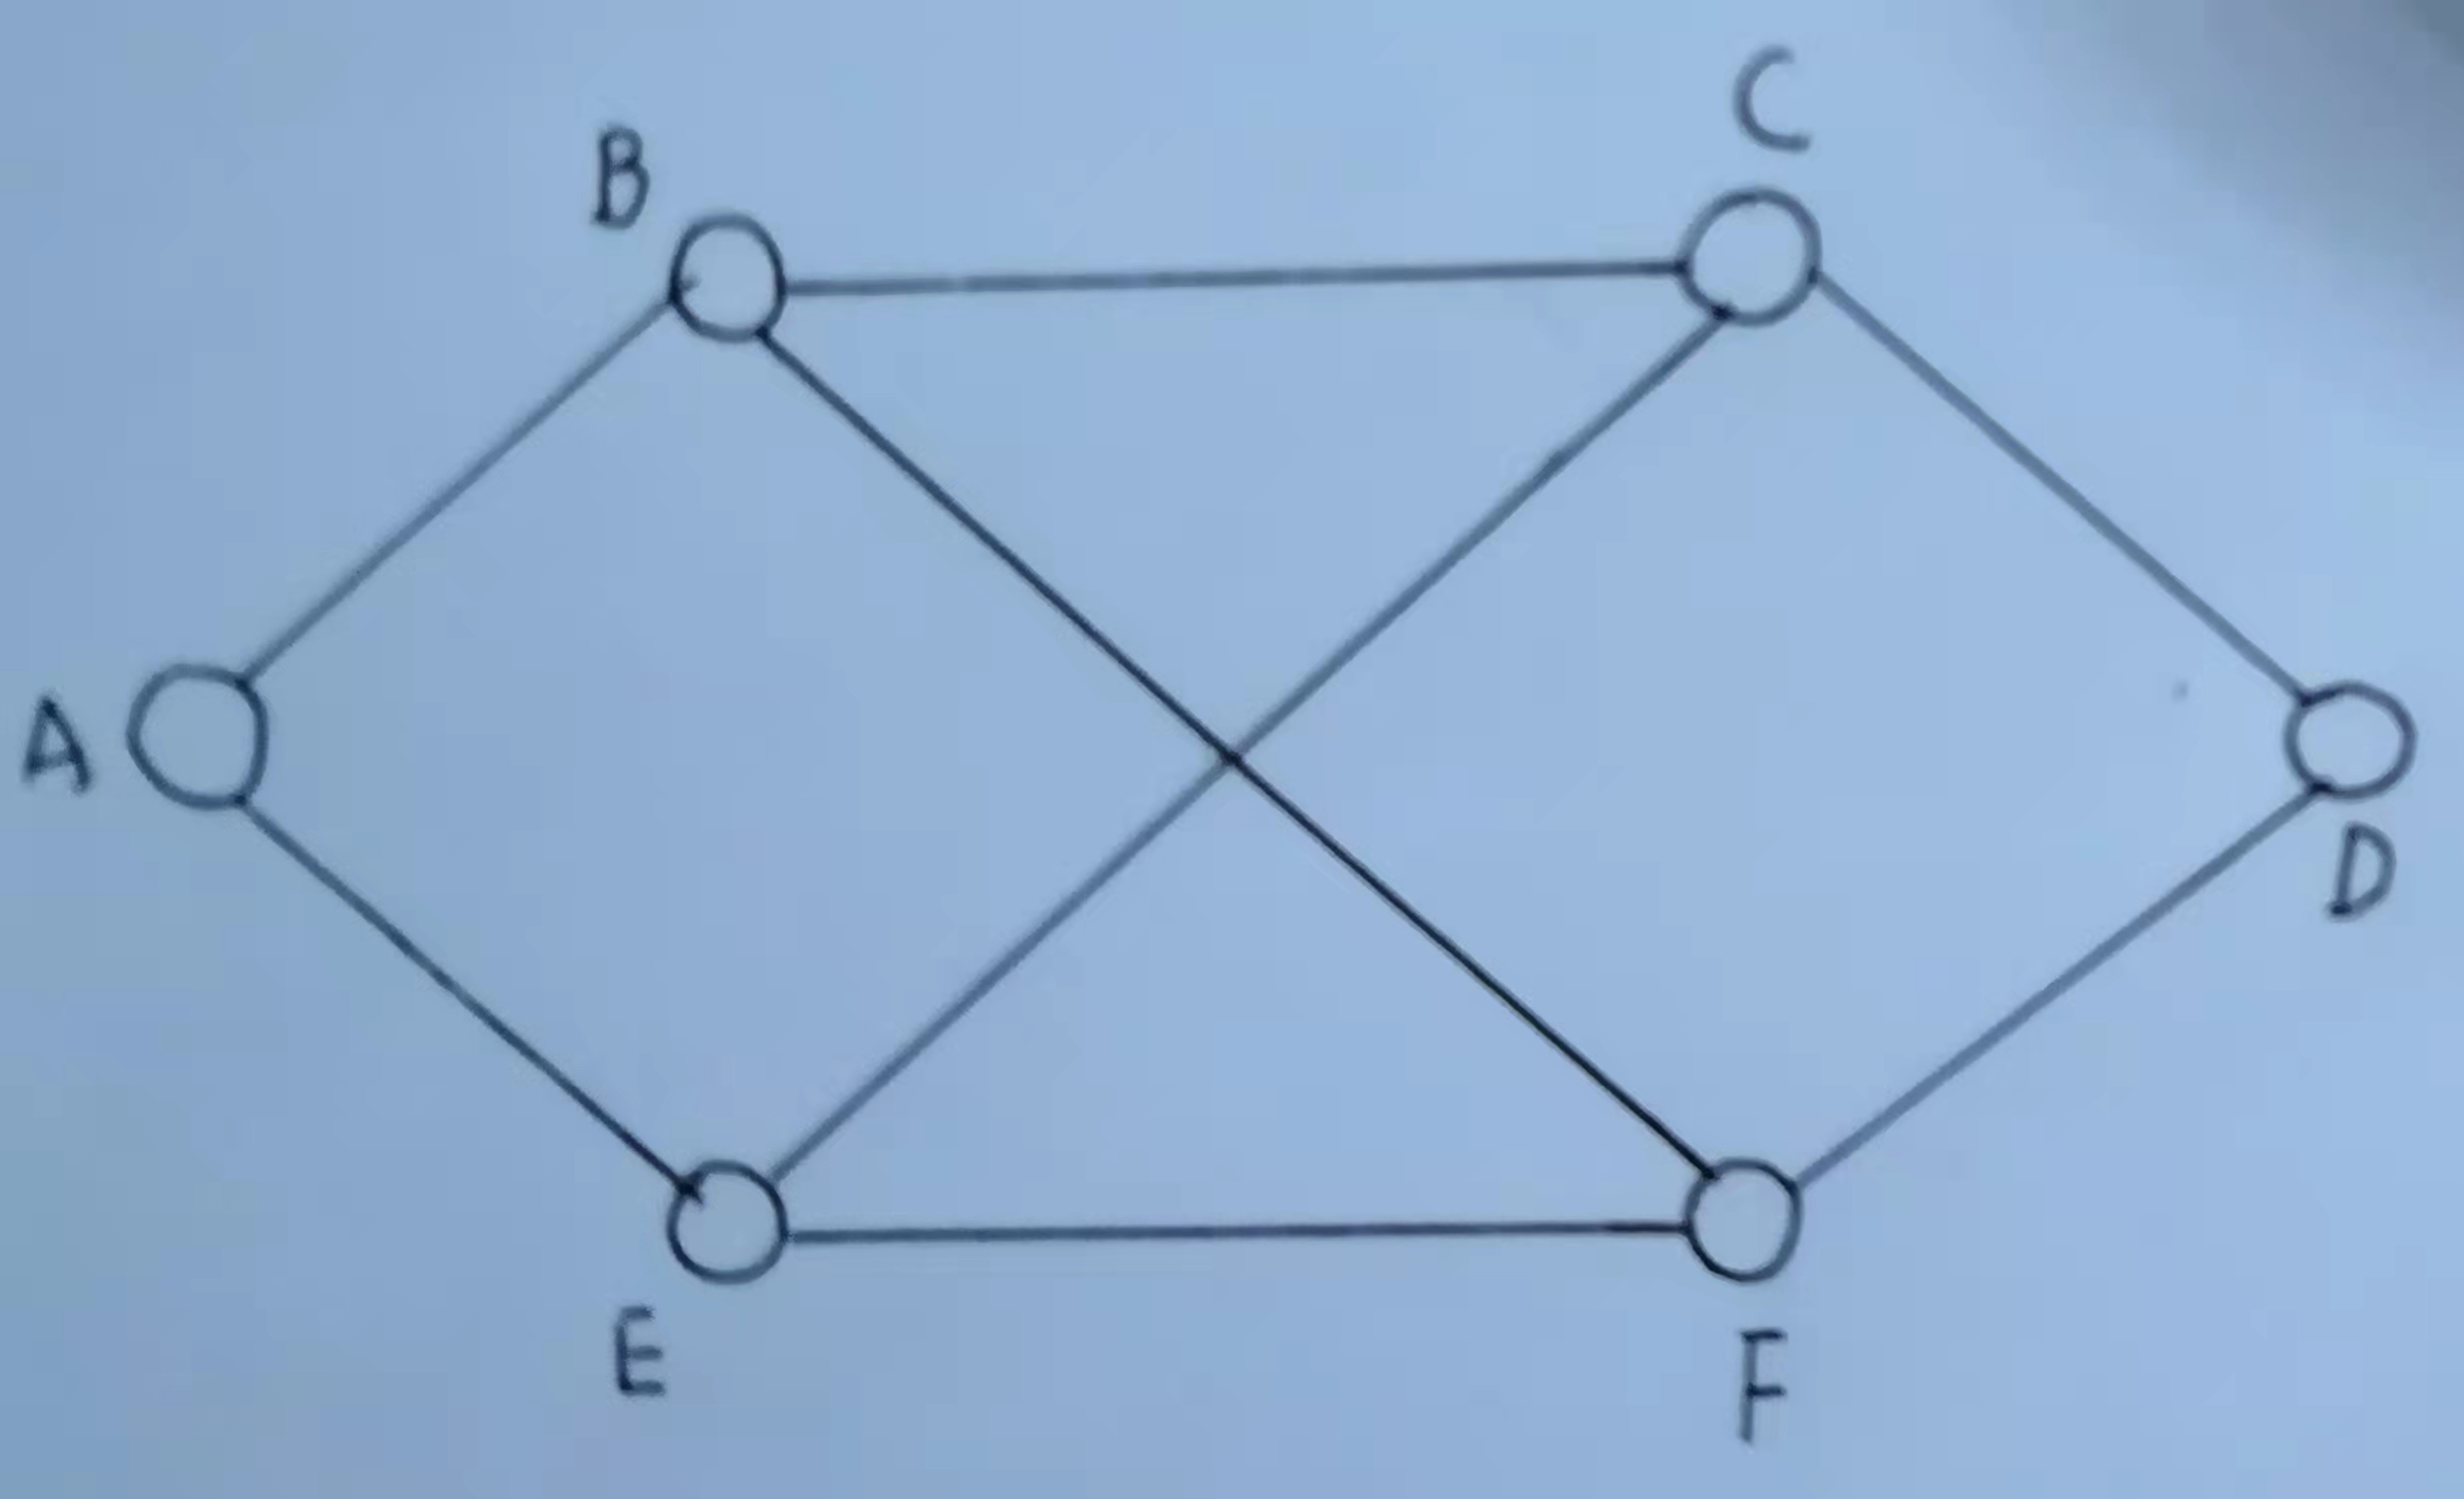
\includegraphics[width=4cm,height=4cm]{8.jpg}
\end{figure}
9.某加性噪声信道的信道模型为$y=x+z,z\sim exp(1)$,即z服从均值为1的指数分布,$x\sim
  \begin{pmatrix}
    0   & A   & 2A  & 3A  \\
    p_1 & p_2 & p_3 & p_4 \\
  \end{pmatrix}$,试根据最大后验概率准则给出判决门限。\\
10.{\color{red}原图比较模糊,建议直接看图片}
\end{document}